\documentclass{article}
\usepackage{fancyhdr} % Required for custom headers
\usepackage{lastpage} % Required to determine the last page for the footer
\usepackage{extramarks} % Required for headers and footers
\usepackage{graphicx} % Required to insert images
%\usepackage{lipsum} % Used for inserting dummy 'Lorem ipsum' text into the template
\usepackage{amsmath}
%\usepackage{amsfont}
%\usepackage{amssymb}

\usepackage{multicol}
% Margins
\topmargin=-0.5in
\evensidemargin=0in
\oddsidemargin=-0.5in
\textwidth=7.5in
\textheight=9.0in
\headsep=0.25in 


\pagestyle{fancy}

\rhead{M. Adam} % Top right header
\lhead{Egg Sandwiches}
\chead{ }
%\title{}

\begin{document}
%
%PRELIMINARIES:
%
%
%Begin by preheating the oven to 350 $^o$F
%
%\bigskip
%
%\bigskip

\begin{multicols}{2}
Ingredients:
\begin{itemize}
\item 6 eggs
\item 1/3 cup mayonnaise
\item 2-3 gherkins, chopped
\item 1 small shallot or ¼ red onion
\item 1/2 bunch of chives
\item Salt and pepper to taste
\item Bread for serving
\end{itemize}

\columnbreak

Directions:
\begin{enumerate}
\item Place eggs in a small pot of cold water on the stove over medium heat.

\item Once the water starts boiling, allow the eggs to boil for about 12-15 minutes.

\item Remove eggs from the water and allow them to cool (can be placed in the fridge).

\item Peel the shells off the egg and place them in a bowl and mash them into small chunks with a fork.

\item Add your mayonnaise, freshly chopped shallots, your chopped gherkins or pickles and half of the freshly chopped chives. Add salt and pepper to your liking and mix all the ingredients together.

\item Scoop small amounts of the egg mix onto ½ slices of bread (I use gluten-free bread) and garnish with a few chopped chives.

\end{enumerate}
\end{multicols}



\begin{center}
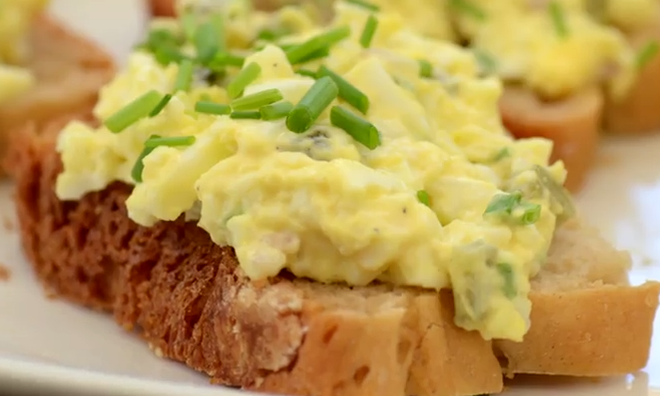
\includegraphics[scale=0.4]{EggSandwiches.png}
\end{center}


\end{document} 











